\chapter{Resultados y Análisis}

Para este capitulo se propone una habitación modelo, con la cual se describen ciertos pasos y funcionamientos de la solución en general. En la figura XXXX esta el esquema de la solución IoT, para esto se supone una habitación con un sensor de temperatura, un ventilador y un bombillo led, las cuales el usuario va a visualizar y gestionar desde la aplicación web.

\section{Software}

Se desarrolla la aplicación web de manera local y posteriormente se lanza a un servidor en Internet. Se encuentra compuesta por los siguientes sitios y las diferentes interacciones basadas en las funciones básicas, crear, leer, actualizar y borrar (CRUD).

\begin{itemize}
	\item Parte Pública
	\item Parte Privada
	\begin{itemize}
		\item API
		\item Panel de Control
		\begin{itemize}
			\item Crear
			\item Ver
			\item Editar
			\item Eliminar 
		\end{itemize}
	\end{itemize}
\end{itemize}

De acuerdo a la lista anterior, se toman en cuenta dos partes para esta, una pública y una privada, como se observa en la figura \ref{fig:index}. En la parte pública se encuentra una vista con los datos de contacto, solicitudes de registro o productos y la cantidad de usuarios que actualmente estan registrados en la aplicación. En la parte privada se encuentra la interacción de los usuarios sea administrador, dueño de una casa o de una habitación, para controlar y ver sus datos.\\

Las diferentes interacciones que tiene cada usuario en el panel de control se garantizan por medio del framework, creando diferentes roles para cada usuario que se esta registrando y realizando la comprobación por parte de los controladores y el middleware que este provee.\\

\begin{figure}[H]
\centering
\caption{Página de Inicio}
\label{fig:index}
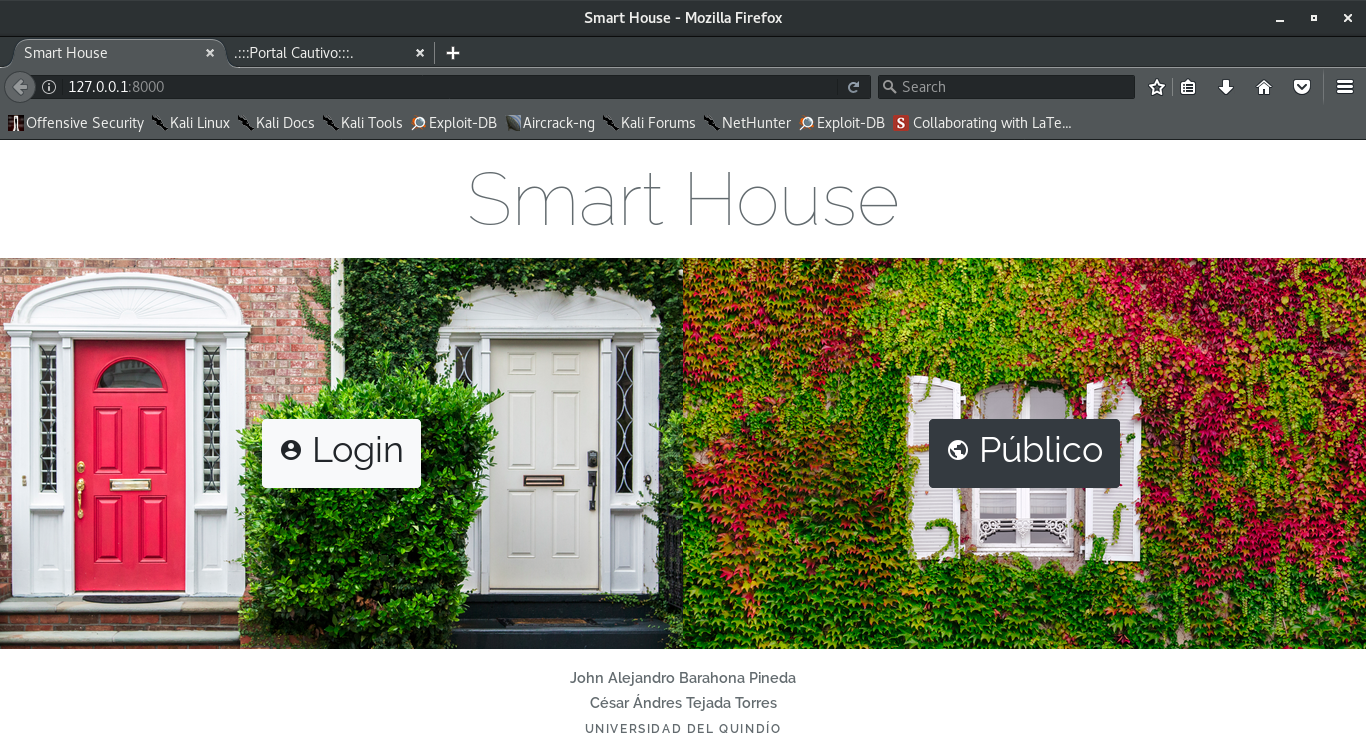
\includegraphics[width=0.9\linewidth]{Imagenes/Index}
\end{figure}

\subsection{Parte Pública}

En esta vista unicamente hay opciones para el contacto y solicitudes, como se menciona anteriormente, es una vista sencilla dada la poca información que contiene, como se observa en la figura \ref{fig:publicview}.

\begin{figure}[H]
\centering
\caption{Vista Pública}
\label{fig:publicview}
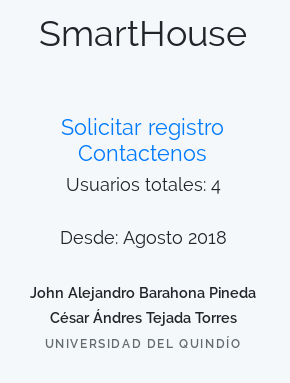
\includegraphics[width=0.9\linewidth]{Imagenes/Public_view}
\end{figure}

\subsection{Parte Privada}

En esta sección es donde se encuentra el Panel de Control para los diferentes usuarios de la aplicación. En primera instancia, para un usuario administrador, que es el encargado de gestionar la aplicación, este usuario tiene la posibilidad de crear, ver, editar y eliminar los diferentes registros de la aplicación, la vista de este usuario se puede observar en la figura \ref{fig:adminview}. Por medio de este usuario es que se activan las cuentas de los demás, por esto en la parte pública estás las opciones de contacto y solicitud de registro.\\

\begin{figure}[H]
	\centering
	\caption{Vistas de Usuarios}
	\label{fig:views}
	\subfigure[Usuario Administrador]{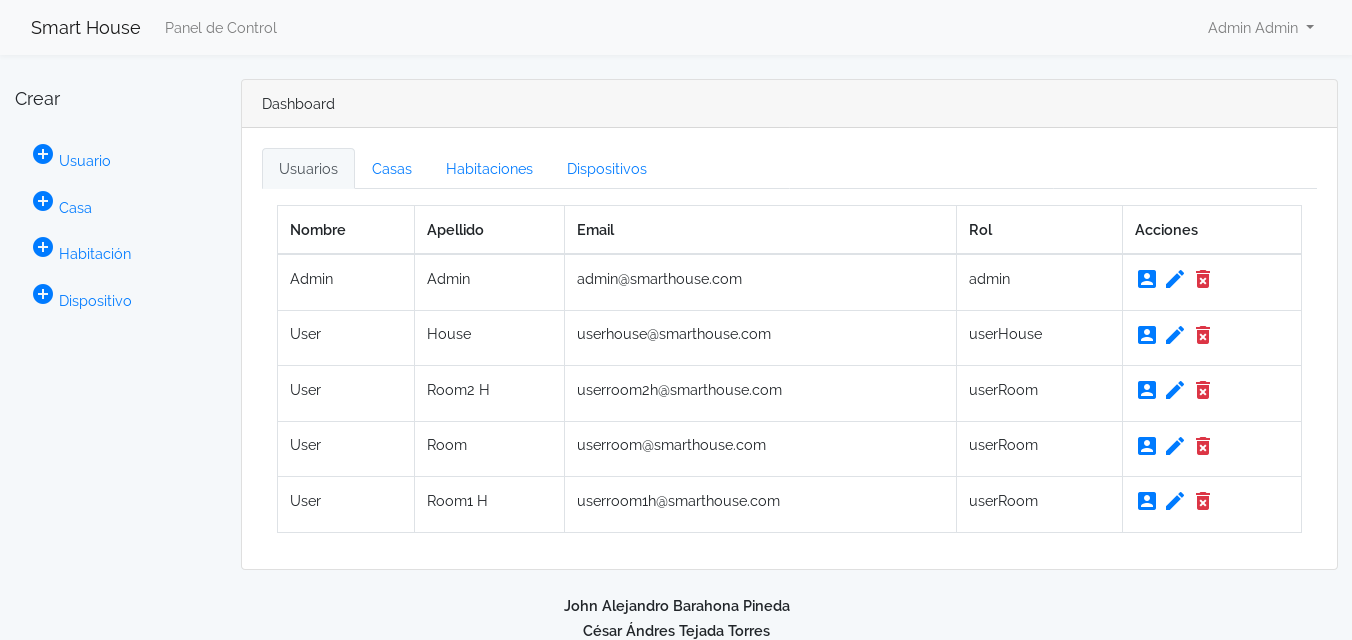
\includegraphics[width=0.9\linewidth]{Imagenes/Admin_view}
		\label{fig:adminview}}
	\subfigure[Usuario de Casa]{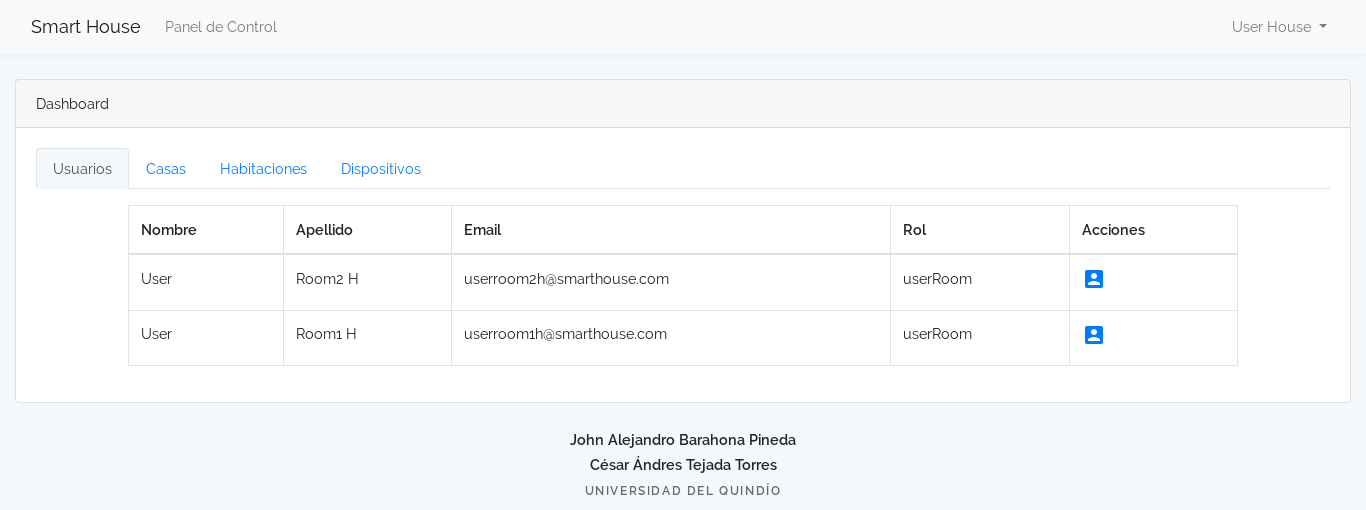
\includegraphics[width=0.45\linewidth]{Imagenes/UserH_view}
		\label{fig:userhview}}
	\subfigure[Usuario de Habitación]{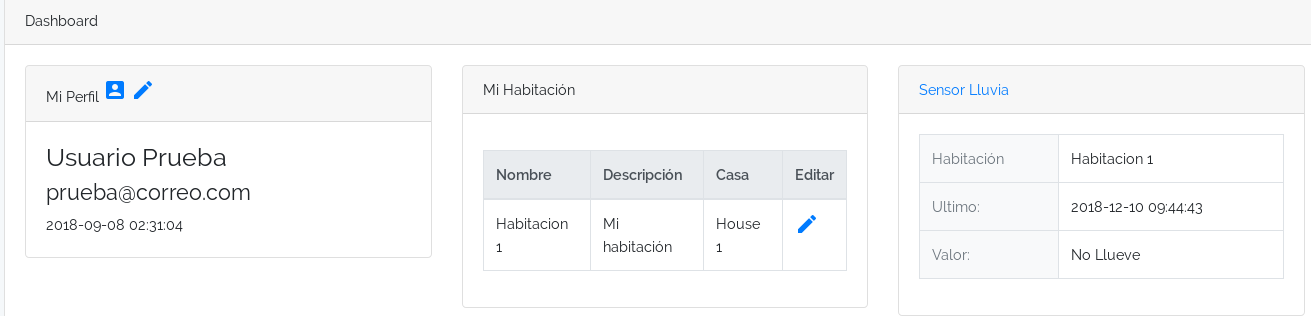
\includegraphics[width=0.45\linewidth]{Imagenes/UserR_view}
		\label{fig:userrview}}
\end{figure}


También existe el usuario dueño de la casa donde se encuentra el dispositivo, este usuario es opcional y es para gestionar los dispositivos presentes dentro de una misma casa, es un administrador de la casa, el cual puede ver y editar algunos campos de sus usuarios hijos o usuarios habitación y sus diferentes casas y habitaciones, unicamente las que esten registradas a su nombre, como se ve en la figura \ref{fig:userhview}, de este modo el rol de este usuario es administrar su casa y visualizar los datos de esta.\\

Por último, otro rol es el de usuario habitación, el cuál es un usuario que solo visualiza sus propios datos, como la habitación y los dispositivos presentes en esta, como se observa en la figura \ref{fig:userrview}, a este solo le compete la información de lo que posee en su habitación, por tal motivo el panel de control muestra una vista general de los datos y el estado de sus dispositivos, además de tener la capacidad de editar partes básicas de su habitación y perfil. Este usuario puede o no estar sujeto a un usuario padre o usuario casa, ya que, solamente puede poseer una tarjeta para su habitación y ninguna otra en dicha casa.\\

Continuando con este usuario y la habitación modelo propuesta al inicio del capitulo, luego de que el usuario accede a la aplicación web e inicia sesión con los datos que ha registrado en el sistema, al ser un usuario de una habitación, este se encuentra con un panel de control como el de la figura \ref{fig:userhview}, allí puede gestionar los dispositivos presentes en su habitación, así pues, puede visualizar la temperatura que se ha sensado y también encender o apagar los dispositivos conectados a la tarjeta.\\

Además de este panel de control, desde el cuál se realizan las operaciones sobre la aplicación, en la parte privada se encuentra la ruta encargada de la actualización Servidor-Tarjeta, es decir, en esta ruta es donde se da la comunicación. En esta ruta se realiza una petición HTTP tipo GET por parte de la tarjeta, esta contiene el id de la habitación en la cuál esta instalada la tarjeta y también el token correspondiente a esta, y además en la URL se añade un texto tipo JSON en el cual se encuentra toda la información de la lectura actual de los sensores, esta petición la responde el servidor con un texto, también tipo JSON que contiene la información pertinente de las cargas o actuadores, como se observa la figura \ref{fig:updateview}, para dar seguridad a esta transacción, se se utiliza el token mencionado anteriormente, el cual se verifica mediante el id de la habitación y que este coincida con los datos almacenados, de este modo se garantiza que lo que se envía este sometido a verificación.\\

\begin{figure}[H]
	\centering
	\caption{Página de intercambio de datos}
	\label{fig:updateview}
	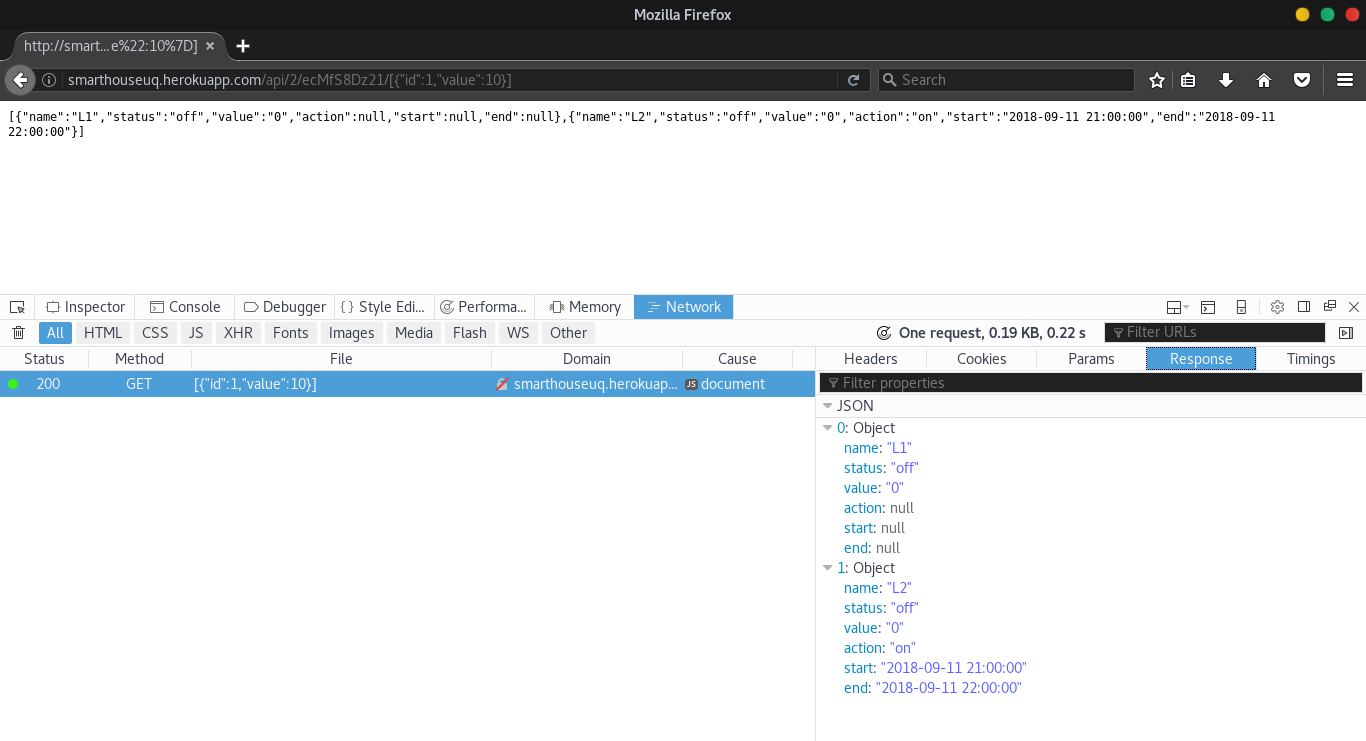
\includegraphics[width=0.85\linewidth]{Imagenes/Update_view}
\end{figure}

De este modo, el usuario interactuando con la aplicación genera modificaciones en el texto con que responde la aplicación web a la petición de la tarjeta. Si el usuario desea encender el ventilador, como se observa en la figura \ref{fig:userhview} esta presente un botón en la información del dispositivo, el cual con presionarlo lo enciende o apaga, esto es valido para cualquiera de los dos dispositivos, sea el ventilador o el bombillo led.\\

Si el ventilador esta conectado a una salida de AC controlada es posible que por medio del deslizador se le asigne un valor para que cambie su funcionamiento, del mismo modo para el bombillo led donde se refleja en su cambio de intensidad, pero este conectado a una salida DC controlada. Al generar estas interacciones el texto en formato JSON cambia de acuerdo a lo pedido por el usuario.\\ 

También si el usuario desea añadir, modificar o eliminar una regla, por ejemplo, desea encender el bombillo led a una hora deseada, esto lo puede lograr mediante el botón de reglas en el panel de control, el cual lo redirige a la vista que se observa en la figura \ref{fig:rulesview}, en esta se indica una hora de inicio y finalización en la cual el bombillo led enciende a la hora de inicio y se apaga a la hora de fin, si es la regla de apagado solo necesita una hora de inicio para apagar el bombillo.

\begin{figure}[H]
	\centering
	\caption{Vista para añadir reglas}
	\label{fig:rulesview}
	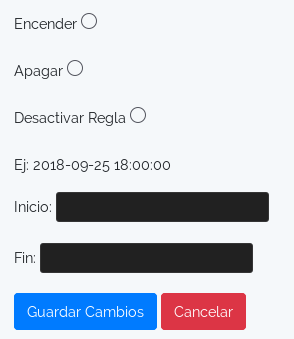
\includegraphics[width=0.6\linewidth]{Imagenes/rules_view}
\end{figure}

\subsection{Base de Datos}

La estructura de la base de datos se puede observar en la figura \ref{fig:db}, aquí se observan los diferentes campos que posee cada tabla, además de las llaves y sus relaciones, las relaciones presentes en esta estructura son de tipo 1:N, es decir, por ejemplo un usuario puede tener relacionadas N casas.

\begin{figure}[H]
\centering
\caption{Base de datos SmartHouse}
\label{fig:db}
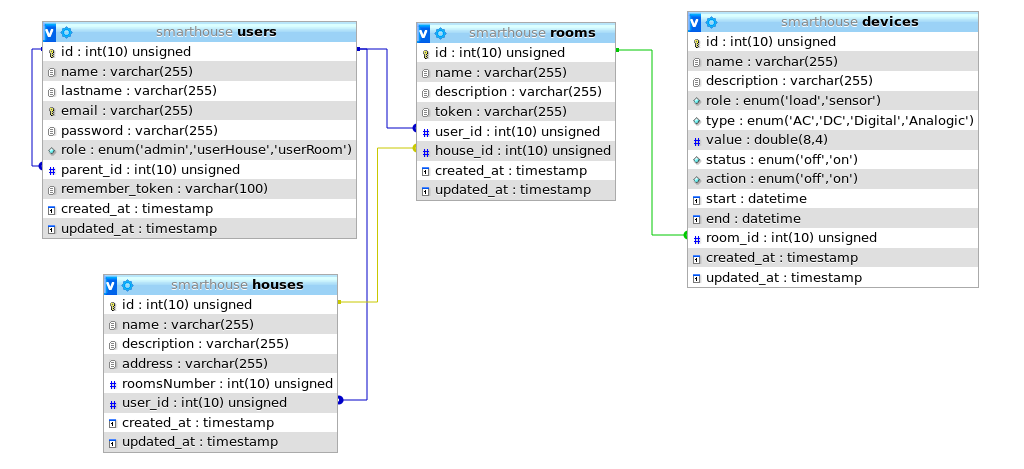
\includegraphics[width=0.7\linewidth]{Imagenes/DB}
\end{figure}

\section{Firmware}

\subsection{Conexión a Internet vía Wi-Fi}

Los sistemas IoT deben estar conectados siempre a Internet, por este motivo se debe brindar una forma para conectar al sistema a este, por lo tanto, se desarrolla un servidor local en la tarjeta que se encarga de esto, como se ha mencionado el módulo del esp32 funciona como Punto de Acceso (AP) y como Cliente o Estación (STA) al mismo tiempo, aprovechando esta capacidad se usa el servidor local y esta encargado de gestionar la conexión de la tarjeta vía Wi-Fi como se observa en la figura \ref{fig:conexion}.\\

\begin{figure}[H]
	\centering
	\caption{Conexión a Internet vía Wi-Fi ESP32}
	\label{fig:conexion}
	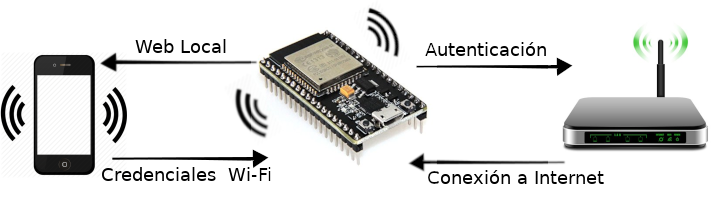
\includegraphics[width=0.7\linewidth]{Imagenes/conexion}
\end{figure}


De este modo, en la figura \ref{fig:wifi} están algunas paginas del servidor local de la tarjeta, en la figura \ref{fig:red} se puede ver la lista de las diferentes redes al alcance de la tarjeta, basta con seleccionar una red e ingresar sus credenciales para conectarse a esta, en la figura \ref{fig:opt} se observan los detalles de la conexión actual y también la opción de desconectarse de esta. Su funcionamiento es muy intuitivo, se selecciona la red a la que se desea conectar la tarjeta, se ingresan sus credenciales y posteriormente el dispositivo verifica si la conexión fue exitosa o no, si la conexión es exitosa ya la tarjeta esta lista para su funcionamiento, se debe reiniciar para que solo quede funcionando como STA y no en el modo dual, además de esto si las credenciales de la red cambian también se incluye un botón para el borrado de estas, para que se puede configurar de nuevo la conexión a la red Wi-Fi.

\begin{figure}[H]
	\centering
	\caption{Aplicación Conexión a Wi-Fi}
	\label{fig:wifi}
	\subfigure[Lista de Redes]{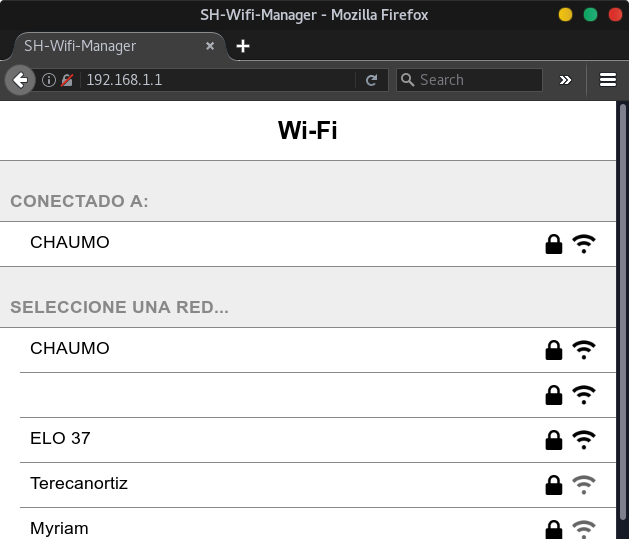
\includegraphics[width=0.45\linewidth]{Imagenes/w_status}
		\label{fig:red}}
	\subfigure[Datos de Conexión]{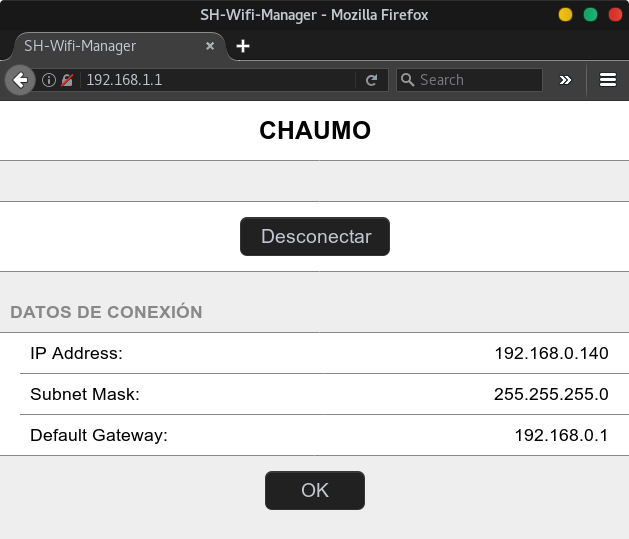
\includegraphics[width=0.45\linewidth]{Imagenes/w_red}
		\label{fig:opt}}
\end{figure}

\subsection{Escritura de Datos en la Aplicación Web}

Los datos que esta leyendo la tarjeta provienen de los diferentes sensores que tiene conectados como se ha mencionado, se usan diferentes tipos, como de estado para sensar la presencia, de calidad de aire entre otros presentes en esta. Para la escritura de los datos, en el firmware, se desarrollan diferentes tareas encargadas de leer y enviar estos a una tarea central. Los datos que están enviando contienen el id del dispositivo y la medida que lee en ese momento, estos se envían en forma de texto en formato JSON, de este modo, la tarea central los gestiona y envía a la aplicación con el mismo formato, organizandolos en la petición HTTP tipo GET que realiza, así la url que la tarjeta solicita, incluyendo el JSON de cada sensor, se observa en la figura \ref{fig:json}, de este modo, en la url se encuentra el dominio del servidor, y la dirección que contiene el id y token de la habitación, por último esta la información del sensor en formato JSON, que se compone por el id y el valor de este. La aplicación ya se encarga de almacenarlos y mostrarlos al usuario como se menciona anteriormente.

\begin{figure}[H]
	\centering
	\caption{URL de la petición HTTP}
	\label{fig:json}
	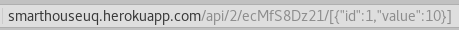
\includegraphics[width=0.7\linewidth]{Imagenes/JSON}
\end{figure}


\subsection{Lectura de Datos de Internet}

Para la configuración y comparación de las reglas que suministra el usuario a el dispositivo que dese controlar es necesario contar con la hora actual y que se siga actualizando localmente gracias al RTC que posee internamente el esp32, así, al inicio de la aplicación, se sincroniza y almacena la hora actual de la red, por medio del protocolo SNTP. Estas reglas actúan en cuanto a que encienda o apague un dispositivo a una hora dada, después de obtener este dato la aplicación continua con normalidad para realizar las diferentes peticiones a la aplicación web.\\

La interacción del usuario se da con la aplicación web mencionada anteriormente, de este modo la tarjeta siempre se debe actualizar, para esto, cuando la tarjeta envía los datos de los sensores la aplicación responde con los datos necesarios para tarjeta, esta los recibe en una cadena texto en formato JSON como se observa en la figura \ref{fig:updateview}, los procesa y envía a las tareas pertinentes ya sea para encender o apagar algún dispositivo conectado a la tarjeta, además envía las reglas que el usuario ha definido.